% Modelo de TCC do Bacharelado em Ciência da Computação da UNIFESP 
% Baseado no Modelo de Documentos Academicos do ABNTex2  

\documentclass[	12pt, Times, openright, twoside, a4paper, english, brazil]{abntex2}

% ---
% Pacotes fundamentais 
% ---
\usepackage{cmap}				% Mapear caracteres especiais no PDF
%\usepackage{lmodern}			% Usa a fonte Latin Modern			
\usepackage{times}
\usepackage[T1]{fontenc}			% Selecao de codigos de fonte.
\usepackage[utf8]{inputenc}		% Codificacao do documento (conversão automática dos acentos)
\usepackage{lastpage}			% Usado pela Ficha catalográfica
%\usepackage{natbib}
\usepackage{indentfirst}			% Indenta o primeiro parágrafo de cada seção.
\usepackage{color}				% Controle das cores
\usepackage{graphicx}			% Inclusão de gráficos
% ---
\usepackage[portuguese, ruled, linesnumbered]{algorithm2e} %Peseudocodigo
\usepackage{amssymb} %checkmarker
% ---
% Pacotes de citações
% ---
\usepackage[brazilian,hyperpageref]{backref}	 % Paginas com as citações na bibl
\usepackage[alf]{abntex2cite}	% Citações padrão ABNT

% --- 
% CONFIGURAÇÕES DE PACOTES
% --- 

% ---
% Configurações do pacote backref
% Usado sem a opção hyperpageref de backref
\renewcommand{\backrefpagesname}{Citado na(s) página(s):~}
% Texto padrão antes do número das páginas
\renewcommand{\backref}{}
% Define os textos da citação
\renewcommand*{\backrefalt}[4]{
	\ifcase #1 %
		Nenhuma citação no texto.%
	\or
		Citado na página #2.%
	\else
		Citado #1 vezes nas páginas #2.%
	\fi}%
% ---

% numeração de figuras e elas 
\counterwithout{figure}{section}
\counterwithout{table}{section}

%\renewcommand\tablename{Tabela{\arabic{chapter}.}}


% ---
% Informações de dados para CAPA e FOLHA DE ROSTO
% ---
\titulo{ANÁLISE DE DEMANDA VIA INTELIGÊNCIA ARTIFICIAL NO RESTAURANTE UNIVERSITÁRIO DO INSTITUTO CENTRAL DE TECNOLOGIA DA UNIFESP}
\autor{Douglas Diniz Landim}
\local{São José dos Campos, SP}
\data{Outubro de 2018}
\orientador{Prof. Dr. Vinicius Veloso}
%\coorientador{Prof. Dr. }
\instituicao{%
  Universidade Federal de São Paulo -- UNIFESP
  \par
  Instituto de Ciência de Tecnologia
  \par
  Bacharelado em Ciência da Computação}
\tipotrabalho{Trabalho de Graduação}
% O preambulo deve conter o tipo do trabalho, o objetivo, 
% o nome da instituição e a área de concentração 
\preambulo{Trabalho de conclusão de curso apresentado ao Instituto de Ciência e Tecnologia – UNIFESP, como parte das atividades para obtenção do título de Bacharel em Ciência da Computação.}
% ---

% informações do PDF
\makeatletter
\hypersetup{
     	%pagebackref=true,
		pdftitle={\@title}, 
		pdfauthor={\@author},
    	pdfsubject={\imprimirpreambulo},
	    pdfcreator={LaTeX with abnTeX2},
		pdfkeywords={abnt}{latex}{abntex}{abntex2}{trabalho acadêmico}, 
		colorlinks=true,       		% false: boxed links; true: colored links
    	linkcolor=blue,          	% color of internal links
    	citecolor=blue,        		% color of links to bibliography
    	filecolor=magenta,      		% color of file links
		urlcolor=blue,
		bookmarksdepth=4
}

\makeatother
% --- 
% --- 
% Espaçamentos entre linhas e parágrafos 
% --- 
% O tamanho do parágrafo é dado por:
\setlength{\parindent}{1.3cm}
% Controle do espaçamento entre um parágrafo e outro:
\setlength{\parskip}{0.2cm}  % tente também \onelineskip
% ---

% compila o indice
% ---
\makeindex
% ---

% ----
% Início do documento
% ----
\begin{document}
% Retira espaço extra obsoleto entre as frases.
\frenchspacing 

% ----------------------------------------------------------
% ELEMENTOS PRÉ-TEXTUAIS
% ----------------------------------------------------------
% \pretextual

% ---
% Capa
% ---
\begin{capa}
  \begin{center}
   
\includegraphics[width=.25\textwidth]{logo-unifesp.pdf}
    \vspace*{\fill}
    
    {\ABNTEXchapterfont\large\imprimirautor}
    \vspace*{\fill}
    
    {\ABNTEXchapterfont\bfseries\Large\imprimirtitulo}
    \vspace*{\fill}\vspace*{\fill}
    
   \imprimirlocal
   \end{center}
\end{capa}

% ---
% Folha de rosto
% (o * indica que haverá a ficha bibliográfica)
% ---
\imprimirfolhaderosto*
% ---

% ---
% Inserir folha de aprovação
% ---
% Isto é um exemplo de Folha de aprovação, elemento obrigatório da NBR
% 14724/2011 (seção 4.2.1.3). Você pode utilizar este modelo até a aprovação
% do trabalho. Após isso, substitua todo o conteúdo deste arquivo por uma
% imagem da página assinada pela banca com o comando abaixo:
%
% \includepdf{folhadeaprovacao_final.pdf}
%
\begin{folhadeaprovacao}
  \begin{center}
    {\ABNTEXchapterfont\large\imprimirautor}

    \vspace*{\fill}\vspace*{\fill}
    {\ABNTEXchapterfont\bfseries\Large\imprimirtitulo}
    \vspace*{\fill}
    
    \hspace{.45\textwidth}
    \begin{minipage}{.5\textwidth}
        \imprimirpreambulo
    \end{minipage}%
    \vspace*{\fill}
   \end{center}
    
   Trabalho para apresentar em NOVEMBRO/2018:

   \assinatura{\textbf{\imprimirorientador} \\ Orientador} 
   \assinatura{\textbf{Professor} \\ Convidado 1}
   \assinatura{\textbf{Professor} \\ Convidado 2}
   \assinatura{\textbf{Professor} \\ Convidado 3}
   %\assinatura{\textbf{Professor} \\ Convidado 4}
      
   \begin{center}
    \vspace*{0.5cm}
    {\large\imprimirlocal}
    \par
    {\large\imprimirdata}
    \vspace*{1cm}
  \end{center}
  
\end{folhadeaprovacao}
% ---

% ---
% Dedicatória
% ---
\begin{dedicatoria}
   \vspace*{\fill}
   \centering
   \noindent
   \textit{ Este trabalho é dedicado aos meus pais que apoiaram e sacrificaram esforços para me manter ativo nessa jornada, a todos os professores que me somaram conhecimentos, oportunidades e esperanças indo além de suas rotinas e agendas em prol do ensino, e principalmente à todos que me motivaram me oferecendo desafios para que eu pudesse enfrentá-los superando meus próprios limites } \vspace*{\fill}
\end{dedicatoria}
% ---

% ---
% Agradecimentos
% ---
\begin{agradecimentos}
Minha jornada pela graduação foi marcada por muita persistência, dificuldades e fracassos. Agradeço primeiramente a Deus por me dar fé e alimentar minha persistência e esperança. Apesar de todo o conteúdo técnico das mais de 40 disciplinas do meu curso, o que mais me agregou evolução foi o ambiente extremamente desafiador desta universidade; que somado à muitas dificuldades pessoais, acidentes, contra-tempos de saúde, profissão e família; constituiu a soma perfeita de desafios que me derrubaram muitas e muitas vezes e me fizeram ser uma pessoa melhor, mais convicta e mais perseverante a cada nova tentativa de conquistar minhas aprovações. Agradeço à minha família por sempre me apoiar dando tudo de si, a meu professor por me aceitar orientar, e me motivar sempre me dando atenção como um amigo nas conversas no fim da aula durante o caminho até o estacionamento da faculdade, nas reuniões e chats online até nos finais de semana, aos amigos universitários, e a todos os professores que me acompanharam e ofereceram desafios em todos esses anos na UNIFESP. 

\end{agradecimentos}
% ---

% ---
% Epígrafe
% ---
\begin{epigrafe}
    \vspace*{\fill}
	\begin{flushright}
		\textit{Mesmo desacreditado e ignorado por todos, não posso desistir, pois para mim, vencer é nunca desistir.\\
		(Albert Einstein)}
	\end{flushright}
\end{epigrafe}
% ---

% ---
% RESUMOS
% ---

% resumo em português
\begin{resumo}
O presente trabalho tem como objetivo a comparação com o método de análise da previsão de vendas do restaurante universitário da Unifesp, previamente feita pelo autor deste projeto com aplicação de métodos estatísticos, e atualmente com métodos de aprendizado de máquina. Tal análise por aprendizado de máquina foi apontado como relevante solução no fim da análise estatística do trabalho anterior. A temperatura da região onde se localiza o campus do restaurante foi analisada por recorrência via bootstrap como um fator que exerce impacto sobre as vendas do restaurante em certos períodos do semestre, e neste trabalho de conclusão de curso serão obtidas novas variáveis e um intervalo maior de amostragem na análise da previsão de demanda de refeições do restaurante em um novo modelo com aprendizado de máquina a fim de que seja obtido um modelo de previsão viável para evitar super-projeção de demanda com consequência de desperdício de alimentos, ou subprojeção com consequência de docentes ou discentes sem refeições.
 
 \vspace{\onelineskip}
    
 \noindent
 \textbf{Palavras-chaves}: Redes Neurais Artificiais. Previsão de demanda. Aprendizado de Máquina. Inteligência Artificial. Perceptron Múltiplas camadas. 
 
\end{resumo}

% resumo em inglês
\begin{resumo}[Abstract]
 \begin{otherlanguage*}{english}

The present work has the objective of comparison with the static method of analysis of the demand prediction in UNIFESP university restaurant, previously done by the author of this project, and currently with machine learning methods. Such analysis by machine learning was pointed out as a relevant solution at the end of the statistical analysis of the previous work. The temperature of the region where the restaurant campus is located was analyzed by bootstrap recurrence as a factor impacting the restaurant sales in certain periods of the semester, and in this work of completion of the course will be obtained new variables and a greater range of sampling in the analysis of the forecast of restaurant meal demand in a new model with machine learning in order to obtain a viable prediction model to avoid overprojection of demand as a result of food waste or subprojection with the consequence of teachers or students without meals.

   \vspace{\onelineskip}
 
   \noindent 
   \textbf{Key-words}: Artificial Neural Networks. Demand Prediction. Machine Learning. Artificial intelligence. Perceptron Multiple layers.
 \end{otherlanguage*}
\end{resumo}

% ---
% inserir lista de ilustrações
% ---
\pdfbookmark[0]{\listfigurename}{lof}
\listoffigures*
\cleardoublepage
% ---

% ---
% inserir lista de tabelas
% ---
\pdfbookmark[0]{\listtablename}{lot}
\listoftables*
\cleardoublepage
% ---

% ---
% inserir lista de abreviaturas e siglas
% ---
\begin{siglas}
\item[ICT] Instituto Central de Tecnologia
\item[R.U] Restaurante Universitário
\item[UNIFESP] Universidade Federal de São Paulo
\item[BDMEP] Banco de Dados Meteorológicos para Ensino e Pesquisa

\end{siglas}
% ---

% ---
% inserir lista de símbolos
% ---
%\begin{simbolos}
%  \item[$ \Gamma $] Letra grega Gama
%  \item[$ \Lambda $] Lambda
%  \item[$ \zeta $] Letra grega minúscula zeta
%  \item[$ \in $] Pertence
%\end{simbolos}
% ---

% ---
% inserir o sumario
% ---
\pdfbookmark[0]{\contentsname}{toc}
\tableofcontents*
\cleardoublepage
% ---

% ----------------------------------------------------------
% ELEMENTOS TEXTUAIS
% ----------------------------------------------------------
\textual

% ----------------------------------------------------------
% Introdução
% ----------------------------------------------------------
\chapter{Introdução}
\section{Contextualização e Motivação}

\paragraph*{} A previsão de demanda é um ponto de extrema importância para qualquer empresa, uma previsão adequada permite o ajuste de todo o seu mecanismo de operações para atender tal demanda com a melhor eficiência possível, maximizando lucros, minimizando perdas, e principalmente atendendo todas as necessidades do cliente.

\paragraph*{} Todo restaurante universitário enfrenta problemas de previsão de demanda de refeições e prejuízos com a falta de vendas e ou o descarte de refeições não vendidas. Um dos grandes problemas enfrentados hoje no mundo é a elevação dos preços dos alimentos, o valor além de monetário é moral, a alimentação é o recurso primitivo de base da humanidade que hoje ainda enfrenta um mal acesso a este em muitas regiões carentes. O descarte indevido de alimentos, provocado por suas limitações e durabilidade não gera somente prejuízos monetários e sim prejuízos ambientais e morais. Isso tem causado preocupações para a população em geral e também para empresas como restaurantes que sofrem diretamente os reflexos da variação no preço dos alimentos e na demanda. Atualmente o restaurante universitário do ICT - UNIFESP não possui um sistema que ajude na gestão de compras dos alimentos.

\paragraph*{} No restaurante universitário do ICT UNIFESP as refeições são fornecidas de segunda a sexta feira. O caso particular de restaurantes universitários envolve um fluxo de demanda influenciadopor dia da semana, visto que a demanda é influenciada pela quantia de alunos presentes na universidade, que por sua vez é influenciada pela grade de aulas determinada semestralmente por dia da semana. O caso de análise para este projeto foi motivado após informações de relevantes desperdícios.

Devido às condições burocráticas no ambiente do restaurante que compreendem fidelidade de contrato, exclusividade na região pois o restaurante se encontra em localização que o faça ser o único provedor de alimentos ao público do campus estando isolado fisicamente de qualquer região comercial, e acessibilidade do público à aquisição de refeições que em sua maior parte adquirem refeições pelo valor de 2,50 sendo o restante do custo da refeição subsidiada pela instituição através de verbas federais, a escolha dos parâmetros não será influenciada por muitos fatores externos como concorrência, acessibilidade do ponto, entre outros.

\paragraph*{} Outro ponto importante é a obtenção dos valores de venda; não foram escolhidas as vendas diretas do ponto de venda de tickets de refeição, e sim os dados de coleta da entrada do restaurante, que demonstram a real movimentação de público no restaurante em determinado dia.

\paragraph*{} O estudo da relação de vendas, temperatura, outras variáveis climáticas e do ambiente, já é comum em outros cenários, entre eles o de maior destaque é na demanda de energia elétrica. Os cenários de vendas de alimentos perecíveis ganha também destaque apesar de se encontrar investimentos maiores na indústria de produção de energia elétrica. O objetivo tanto no cenário deste trabalho, o restaurante universitário, como em outros cenários é o mesmo, atender toda a demanda de consumo e evitar transtorno à qualquer consumidor pela falta da mesma, e evitar prejuízos de produção não consumida. Tais prejuízos impactam não só ao fornecedor, mas também ao consumidor, um fornecimento de produto e serviço com um bom planejamento de demanda, poupa recursos ao produtor que podem ser investidos em melhor qualidade de produto, e menor preço ao consumidor a fim de que seja obtido um modelo de previsão viável para evitar sobrestimação de demanda com consequência de desperdício de alimentos, ou subestimação com consequência de docentes ou discentes sem refeições. 

\paragraph*{} Tal problema tem sido impactante e frequente para o restaurante que informa que em alguns
dias no mês passa por sobrestimação e desperdício superior a 100 refeições. 

\section{Definição do problema}
O problema a definir neste trabalho é encontrar um modelo de previsão de demanda através de algoritmos de regressão por aprendizado de máquina.

\section{Justificativas}
As atuais abordagens de previsão do restaurante universitário, que envolvem média aritmética simples e dedução subjetiva são falhos por não serem calculados tendo uma visão ampla de todo um histórico de dados de grande amostragem, e também não cruzam informações diversas como dados climáticos, dados de calendário anual, feriados próximos, entre outros.

\section{Objetivos}
\subsection{Objetivo geral}
Construir um modelo utilizando uma Rede Neural Artificial para a previsão da demanda de
refeições do restaurante universitário do ICT-UNIFESP com menos de 10% de erro.
\subsection{Objetivos específicos}
\begin{itemize}
\item Construir modelos utilizando três algoritmos de regressão; 
\item Realizar análise estatística da qualidade dos modelos;
\end{itemize}

\section{Metodologia}
\paragraph*{Estudo de análise de regressão} Por se tratar de um trabalho de previsão de demanda, a primeira atividade será o estudo da tarefa de análise de regressão com foco na previsão de demanda. Análises de regressão fundamentadas por BOCANEGRA (2002) e técnicas aplicadas de regressão propostas por SMOLA (1998), são as principais bases de fundamentação dos trabalhos de previsão de demanda de LOPES(2008) no restaurante universitário da Universidade Federal de Viçosa, e de RUAS et al. (2012) na previsão de demanda de energia elétrica utilizando redes neurais artificiais e regressão por máquinas de vetores de suporte, respectivamente. A partir destes trabalhos, serão estudados diferentes métodos de regressão e como a partir deles podem ser aplicadas técnicas de previsão de demanda por meios estatísticos e usando técnicas de aprendizado de máquina.

\paragraph*{Estudo de Aprendizado de máquina}
Após essa etapa, será então iniciado o estudo aprofundado sobre Redes Neurais Artificiais de acordo com BRAGA (2000), e o estudo específico da técnica de Perceptron Multi-Camadas fundamentado em HAYKIN (1994) que embasa o trabalho realizado na Universidade Federal de Viçosa.

\section{Organização do documento}
Este trabalho está organizado da seguinte forma: o capítulo 2 apresenta os conceitos básicos para o entendimento do trabalho. O capítulo 3 apresenta trabalhos relacionados. O capítulo 4 demonstra o plano de atividades para o TCC II. O capítulo 5 conclui este trabalho.
% ----------------------------------------------------------
% Fundamentação Teórica
% ----------------------------------------------------------
\chapter{Fundamentação Teórica}
\section{Introdução}
A previsão da demanda é o fator principal da eficiência de qualquer modelo de processamento do tipo entrada-saída, onde a sua saída deve atender uma demanda não determinística. É necessário prever a demanda para projetar e aperfeiçoar o processamento e a entrada deste modelo. 

O modelo a ser analisado neste trabalho é o comportamento dos consumidores de um restaurante universitário, onde o mesmo precisa projetar sua compra de insumos e alocação de recursos na entrada de seu modelo de negócio, e projetar sua saída, que é a produção de refeições em quantidade numérica e inteira distribuída em função do tempo em dias, para atender um consumo feito por alunos, que não se comporta de maneira determinística, já que este consumo é facultativo aos alunos.

De acordo com o contrato presente entre o restaurante e a universidade, o mesmo deve atender totalmente à demanda do público, sendo multado se caso algum consumidor fique sem alimentação, porém este mesmo contrato não trata refeições que não são consumidas, logo o restaurante deve lidar integralmente o prejuízo de refeições produzidas acima da demanda de consumo.

Tais refeições fornecidas à alunos também são em parte subsidiadas, no atual ano de 2018 o aluno paga ao restaurante o valor de 2,50 e a Universidade paga a diferença de R\$2,50 reais do custo total da refeição que é R\$13,00 cobrado pelo restaurante, logo esta previsão de demanda corresponde também aos interesses da administração do campus local, que periodicamente deve realizar uma alocação de recursos financeiros para subsidiar todas estas refeições consumidas.

É necessário então entender e descobrir quais elementos influenciam este consumo humano, de que forma estes elementos exercem tal influência e em qual intensidade ela ocorre.

E para explorar tais elementos, é necessário explorar como este consumo ocorreu historicamente a fim de se encontrar padrões de comportamento, que no cenário deste trabalho acontece com informações distribuídas através do tempo. 

Neste capítulo o principal objetivo é definir todos os conceitos que serão necessários para o entendimento total deste trabalho, analisando a forma que os dados são entendidos, e as ferramentas com os quais possam ser trabalhados.

\section{Dados}
Abstraindo o histórico de vendas do restaurante, temos 2 tipos de dados principais. A venda podendo ser uma observação Y, e a data da venda sendo uma observação X. Se comportando de modo que a função de X implica em Y. 

X,Y $\rightarrow Y \simeq f(X) $

A observação principal a ser analisada neste trabalho é o numero de vendas do R.U do ICT - UNIFESP, em valor inteiro, obtido de um dia letivo, em um determinado período sendo este o almoço ou jantar.

O tempo, onde a informação principal se distribui, é em formato de data, e contém apenas 1 valor da venda total de almoços nesta data, e da venda total de jantas nesta data.

\subsection{Dados de Consumo}
Os dados históricos de consumo no restaurante foram retirados do atual sistema banco de dados de refeições subsidiadas do Hospital São Paulo, que gerencia os dados dos refeitórios de todos as unidades da Unifesp. É importante ressaltar que tais dados são apenas de funcionários, docentes e discentes da instituição. Eventuais compras de refeições realizadas por visitantes que não possuem vínculo com a instituição não são registradas pelo sistema. 

Outro fato importante é que estes dados registrados no banco, são registrados no momento em que a refeição é realizada, pelos terminal da entrada do refeitório e não no momento que é vendida pelo caixa do refeitório. Caso fossem registrados no momento da venda no caixa, a análise estatística do consumo poderia sofrer um viés errôneo em relação à frequência de pessoas no refeitório. 

Os alunos são os que realizam o maior volume de consumo, e são os que tem um padrão de frequência à universidade de modo estocástico, que tende a ter uma sazonalidade anual de frequência na universidade desde 2017, quando a instituição padronizou a grade horária de disciplinas.  Além de ser o objetivo principal da previsão por serem os únicos que têm as refeições subsidiadas, pagando um custo de apenas R\$2,50 por refeição, onde entende-se que este custo pode ter mais forte influência na decisão do aluno realizar uma refeição em comparação à outro discente ou pessoa com vínculo na instituição. Por isso os dados que serão analisados neste trabalho, serão somente da frequência de alunos, e terão como início o ano de 2017. 

Apenas alguns funcionários autorizados tem acesso ao banco de dados do sistema de refeições da instituição, entre eles o fiscal de contrato do restaurante universitário. Para obter tais dados neste trabalho, foi necessário obter uma autorização com a direção do campus ICT - UNIFESP e em seguida solicitar a exportação dos dados ao fiscal. Os parâmetros dos quais o mesmo consegue realizar a exportação de dados são diversos, porém foi solicitado o formato de valores separados por vírgula que compreendem o ano de 2017 a 2018.

O modelo exportado segue o seguinte da seguinte forma abaixo, contendo o exemplo de 2 datas: 
\begin{algorithm}[H]
"
CONSULTA POR PERÍODO                    ",,,,,,,,,,
"
CAMPUS: SÃO JOSÉ DOS CAMPOS                    ",,,"
RU: TODOS                    ",,,"
VINCULO: ALUNO                    ",,"
PERÍODO DE: 01/01/2017 A 31/10/2018                        ",,
DATA,VENDAS CAFÉ,VENDAS ALMOÇO,VENDAS JANTAR,VENDAS REFEIÇÃO*,TOTAL VENDAS,ENTR. CAFÉ,ENTR. ALMOÇO,ENTR. JANTAR,TOTAL ENTR. REFEIÇÃO*,TOTAL ENTRADA
(31/10/2018),0,395,0,395,395,0,362,0,362,362
(30/10/2018),0,667,0,667,667,0,437,256,693,693
\end{algorithm}

Logo, no exemplo da segunda linha deste modelo de dados, serão analisados o primeiro valor "(30/10/2018)" como a primeira variável de entrada que corresponde à data, o oitavo valor "437" que corresponde à variável de saída do total de almoço, e ao nono valor "256" que corresponde à variável de saída do total de janta.

Em todo os bancos de dados gerenciados pelo setor de tecnologia da informação da Unifesp, do campus ICT, o mesmo informou que foi constam 428620 refeições subsidiadas no banco de dados do sistema antigo, no período de 2011 à 2016, e 145464 refeições no período de 2017 a 31/10/2018, totalizando 574084 refeições subsidiadas. Generalizando para o valor médio atual de R\$13,00 por refeição recebido pelo restaurante, estima-se então que R\$7.463.092,00 já foram faturados pelos estabelecimentos contratados pelo ICT-UNIFESP, enquanto a mesma subsidiou R\$6.601.966 deste total.

É importante observar que na implementação computacional das análises de predição, o campo de data deve ser convertido à um fator de formato não quantitativo, e a informação do ano /2017 por exemplo deve ser subtraída para a generalização de um modelo de previsão que se adeque à outros anos. Já os campos de número total de refeições consumidas, devem constar como formatos quantitativos nas estruturas de dados dos algoritmos a serem implementados.

Informações derivadas da data não necessitam de coleta, como por exemplo dia da semana, pois podem ser obtidas por métodos de cálculos, sabendo-se apenas um dia da semana correspondente à um dia do ano, ou utilizando bibliotecas computacionais, no caso a biblioteca datetime para a linguagem python.

Para a obtenção de feriados e recessos do calendário acadêmico de um ano determinado, a informação deve ser obtida através do link oficial da instituição, http://www.unifesp.br/reitoria/prograd/pro-reitoria-de-graduacao/informacoes-institucionais/calendario-academico. A única forma de exportação desta informação é em pdf e em formato não tratável facilmente por algoritmos. Então os dias de recesso respectivos ao campus ICT-UNIFESP devem ser carregados manualmente nos códigos a serem implementados.

\subsection{Dados Climáticos}
Também serão analisadas variáveis climáticas juntos com os dados de consumo, de forma a analisar a influência de fatores externos como temperatura média ambiente e precipitação. Tais dados podem ser obtidos de forma gratuita pelo BDMEP - Banco de Dados Meteorológicos para Ensino e Pesquisa, pertencente à instituição pública INMET - Instituto Nacional de Meteorologia, pertencente ao MINISTÉRIO DA AGRICULTURA, PECUÁRIA E ABASTECIMENTO do Governo Brasileiro. 

É necessário um cadastro no site http://www.inmet.gov.br/portal/index.php?r=bdmep/bdmep para a obtenção dos dados. 

A instituição contêm dados registrados de forma digital desde 1961 no país inteiro, os dados históricos referentes a períodos anteriores a 1961 ainda não estão em forma digital e, portanto, estão indisponíveis no BDMEP.

O BDMEP pode fornecer os registros de Precipitação(mm), Temp Máxima(ºC), Temp Mínima(ºC), Insolação(horas)
Evaporação do Piche(mm), Temperatura Compensada Média(ºC), Umidade Relativa Média(\%), Velocidade Vento Média(mps).

Importante ressaltar que o BDMEP leva 90 dias para registrar cada nova data.
Os dados utilizados para este trabalho foram da estação 83781 - São Paulo MIR de Santa - SP.
Observa-se que para futuros trabalhos no atual campus ICT-UNIFESP, a estação TAUBATE - SP 83794, que no momento tem o banco de dados vazio, poderá ser utilizada.

Serão analisadas a temperatura máxima do dia que tem registro em momento próximo à frequência de refeições no horário de almoço, a temperatura mínima do dia que está próxima à janta, e a umidade relativa média que pode indicar presença de chuva no dia, que por sua vez causa diversos impactos ao público da região como a própria frequência do mesmo na instituição, principalmente no fator logístico. 

Os dados se apresentam da seguinte forma: 
\begin{algorithm}[H]
Estacao;Data;Hora;Precipitacao;TempMaxima;TempMinima;Insolacao;Evaporacao Piche;Temp Comp Media;Umidade Relativa Media;Velocidade do Vento Media;
83781;01/01/2017;0000;;31.7;;8.5;6.1;25.2;66;3.466667;
83781;01/01/2017;1200;0;;18.1;;;;;;
83781;02/01/2017;0000;;31.3;;5.6;6.3;23.96;83;2.9;
83781;02/01/2017;1200;16;;18.1;;;;;;
83781;03/01/2017;0000;;31.3;;7;4.5;23.1;87;3;
83781;03/01/2017;1200;3.7;;19.2;;;;;;
\end{algorithm}

Observa-se que cada data contem 2 linhas, sendo a primeira linha com o terceiro campo de valor "0000" apresentando a temperatura máxima do dia no quinto campo, e a segunda linha com o terceiro campo de valor "1200" contendo a temperatura mínima do dia no sexto campo.
A umidade relativa media se encontra no décimo campo da primeira linha de cada data.
Todas as datas apresentam sempre o mesmo padrão de 2 linhas.

\section{Análises Estatísticas}
\subsection{Análise Exploratória dos Dados}
\cite{Junior2007} Cita que dados coletados em modelos de previsão possuem informações que quando são projetadas graficamente evidenciam comportamentos que em alguns casos podem ser visualizados e generalizados de forma subjetiva pelos gestores dos dados.  
Em todos os casos, a análise exploratória é necessária para selecionar o melhor método de análise que se enquadra neste comportamento.

COLOCAR AQUI O GRÁFICO DAS VENDAS DE 2017 / 2018 E AS TEMPERATURAS MEDIDAS.

Somente a análise exploratória não é o suficiente e realizada nos intervalos ou critérios incorretos pode comprometer seriamente as conclusões do comportamento dos dados, e que por sua vez pode comprometer seriamente a decisão dos gestores responsáveis por estes dados, no cenário de uma previsão de demanda. 
Isto ocorre atualmente no cenário de previsão da demanda de refeições do ICT-UNIFESP, onde a universidade e o estabelecimento que fornece as refeições não tem nenhum modelo de previsão de demanda. 

De acordo com o gestor da atual empresa que fornece refeições no ICT, a análise utilizada para se prever as refeições é observar dentro da semana o dia anterior de consumo. Em variações de 300 para 450 refeições aproximadamente, isso tem provocado um desperdício médio de 150 refeições diárias. Em geral, de acordo com o restaurante, todos os dias o mesmo trabalha com um erro e um descarte de 50\% das refeições que são trazidas e consumidas ao campus. Um número estimado de 287.042 refeições descartadas, fornecendo um valor de R\$3.731.546,00 de prejuízo compreendido no período de 2011 a 2018.

\subsection{Métodos de Previsão} 

\cite{Junior2007} Realiza uma revisão bibliográfica extensa abordando principais métodos de previsão de consumo sazonais, no cenário de uma indústria cosmética. Tais métodos estatísticos de previsão se dividem em 2 ramificações, sendo quantitativos ou qualitativos.
Métodos qualitativos fazem um julgamento dos dados expostos sem um sistema de processamento analítico para se produzir novos modelos ou dados, eles são úteis para sistemas de agrupamento, clusterização ou classificação de dados, sem fornecer novas informações numéricas ou modelos preditivos.

Métodos quantitativos que é o foco deste trabalho, são analíticos e se baseiam em um modelo matemático para realizar previsões. 

Para realizar tais previsões os métodos quantitativos necessitam de um histórico de dados, para analisar padrões em seu comportamento e predizer o futuro que irá agir dentro deste padrão.

Estes métodos se ramificam em 2 tipos, as séries temporais e os modelos causais.
\begin{figure}[!ht]
	\center{
		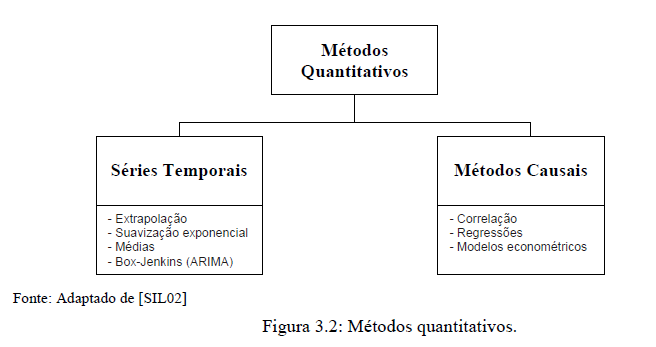
\includegraphics[width=0.65\textwidth]
		{Figuras/JUNIOR2007/metodos-quantitativos.png}
	}
	\caption{Tipos de métodos quantitativos Retirado de \cite{Junior2007}.\label{fig:metodosQuantitativos}}
\end{figure}

\subsection{Métodos de previsão de Demanda}
O autor supracitado também referencia métodos estatísticos especialmente selecionados para uma previsão de demanda, com a atenção de que alguns métodos qualitativos foram criteriosamente selecionados para prever uma demanda industrial, onde geralmente são previstas pelos métodos quantitativos.

\begin{figure}[!ht]
	\center{
		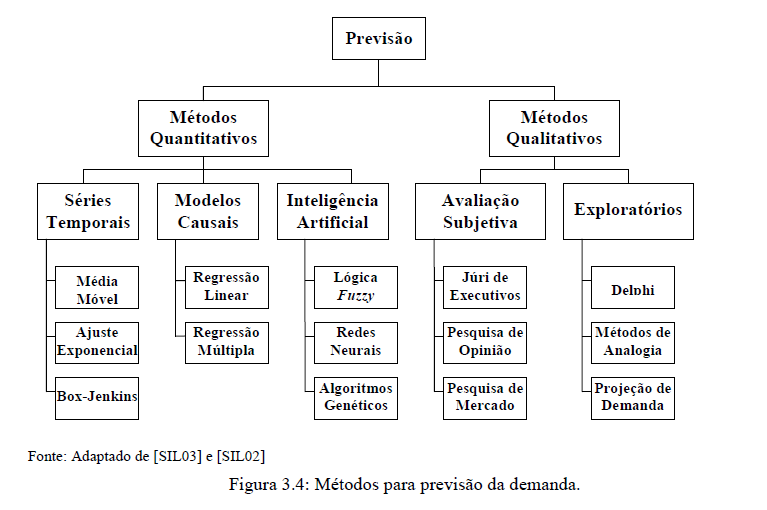
\includegraphics[width=0.65\textwidth]
		{Figuras/JUNIOR2007/metodos-previsao-demanda.png}
	}
	\caption{Tipos de métodos quantitativos Retirado de \cite{Junior2007}.\label{fig:metodosPrevisaoDemanda}}
\end{figure}


\subsection{Meta-análise}
\cite{Flavia2014} cita em sua tese, que resultados e modelos obtidos a partir de análises experimentais em determinado trabalho científico tem a expectativa de confirmação em um padrão de repetição futura, mas que nem sempre tal expectativa é cumprida. Logo é interessante que seja realizado uma análise das análises, ou seja, a comparação de resultados de diferentes métodos obtendo conclusões mais confiáveis e informativas do que o uso único de uma análise.

O comportamento dos dados deste trabalho, apesar de ter uma distribuição de datas, que são em função do tempo e se classificando em um modelo de série temporal, tem tal comportamento impactado por relações causais com outras variáveis como recesso acadêmico, feriados, eventos, precipitações intensas que causam trânsito local e impactam na logística e frequência do público, entre outras variáveis de causas menos aparentes. Portanto será tratado como um modelo de relação causal, implementando o método estatístico de regressão linear, e os métodos de inteligência artificial dos k-vizinhos mais próximos e redes neurais, que serão explicados nos capítulos a se seguir.

\subsection{Séries Temporais}
De acordo com  \cite{Morettin1987} uma série temporal é um conjunto de observações ordenadas em função do tempo, comumente iguais, apresentando uma dependência serial entre elas, sendo um dos objetivos do estudo de séries temporais, analisar e modelar essa dependência. Além disso, séries temporais são analisadas pelos seus principais movimentos, como tendência, sazonalidade e a componente aleatória, sendo a tendencia e sazonalidade as propriedades que mais ganham destaque em pesquisas de previsão de demanda de carga elétrica. Os meios mais comuns de se analisar a componente sazonal são o Método de Regressão (paramétrico), Método de Médias Móveis (não paramétrico), e Método de Diferença Sazonal (sazonalidade determinística).  Neste trabalho, a distribuição dos dados do Restaurante se dá de forma paramétrica, ou seja, as vendas do restaurante se distribuem em função do tempo e com influências de parâmetros como o dia da semana por exemplo, sendo ideal as análises de regressão. 

\cite{Almeida2013} também cita que para realizar a previsão de uma determinada série temporal é possível utilizar diferentes métodos. Pode-se classificá-los basicamente entre métodos estatísticos e baseados em inteligência artificial.
Dentre os métodos estatísticos destacam-se [4]:
- Regressão Linear Múltipla;
- Alisamento Exponencial;
- Média Móvel Integrada Auto-Regressiva (ARIMA)
Entre os métodos baseados em inteligência artificial tem-se:
- Redes Neurais Artificiais;
- Lógica Fuzzy.

\subsection{Componentes Temporais}

É importante observar que os métodos de previsão em séries temporais buscam uma redução da série temporal à um modelo estacionário e à decomposição da série em componentes de tendência, ciclo, sazonalidade e termo aleatório. A tendencia se entende pelo movimento persistente dos dados em uma direção, o ciclo indica o movimento oscilatório desta tendência, sazonalidade indica comportamento regular assumido de forma repetitiva e o termo aleatório se dá por movimentos irregulares presentes na série.
 
As técnicas de previsão para evidências sazonais usam métodos de regressão, que pode ser observados nos trabalhos de previsão de consumo de energia elétrica realizados por \cite{Almeida2013}, \cite{Ruas2012}, \cite{Silva2010} e de previsão de demanda de produtos cosméticos em \cite{Junior2007}

O cenário deste estudo a frequência de alunos dentro do ICT - UNIFESP e consequentemente dentro do R.U tem sazonalidade anual a partir do momento em que a grade de disciplinas foi fixada também com sazonalidade anual. 

\begin{figure}[!ht]
	\center{
		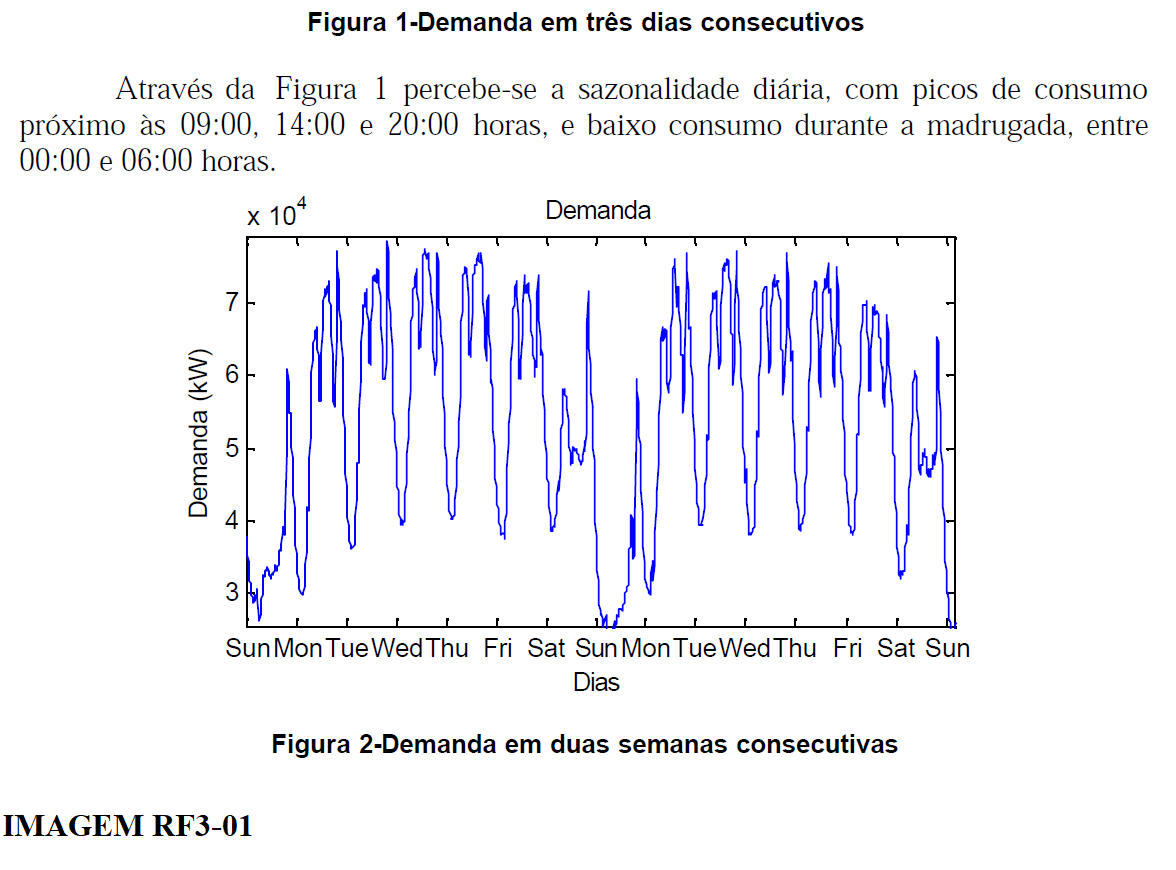
\includegraphics[width=0.65\textwidth]
		{Figuras/RUAS2012/01-DADOS-DE-DEMANDA-EM-FUNCAO-DO-HORARIO.png}
	}
	\caption{DADOS DE DEMANDA DE SAZONALIDADE DIÁRIA, EM FUNÇÃO DO HORÁRIO. Retirado de \cite{RUAS2012}.\label{fig:seriesTemporais}}
\end{figure}

\subsection{Regressão Linear Múltipla}
A teoria da regressão se iniciou no século XIX com Galton, que analisou a altura dos pais e dos filhos (Xi e Yi) e buscou a influencia da altura do pai no filho, notando que a altura do filho tendia à media da altura do pai, e chamou esta técnica de regressão pois existe uma tendência dos dados regredirem à média.

\cite{Clarice2011} informa que em estudos de regressão aplica-se o método relacionar uma variável aleatória Y com outras múltiplas variáveis X. e no caso da regressão simples com apenas uma variável X. 
Ou seja, X,Y $\rightarrow Y \simeq f(X) $

\subsection{Dados espaço-temporais}
Dados espaço-temporais chamados de trajetórias brutas, são coletados através de dispositivos móveis. Uma trajetória bruta é representada por um conjunto de pontos \textit{(tid,x,y,t)}, em que \textit{tid} é o identificador da trajetória e \textit{x, y}, são coordenadas geográficas correspondentes a um lugar no espaço em determinado tempo \textit{t}.

\subsection{Informação}
A informação é o dado analisado e seu contexto ser bem definido compreendendo seus padrões, onde deve-se ter um conjunto de dados a ser processado que podem gerar um valor adicional além dos próprios fatos obtidos.

\subsection{Conhecimento}
Em \cite{Rezende2003}, o conhecimento refere-se à habilidade de se criar um modelo mental que descreva o objeto e indique as ações a serem implementadas e as decisões a tomar. A compreensão e análise se tornam necessárias para a tomada de decisões inteligentes, onde são realizadas a partir do nível do conhecimento obtido através das etapas de obtenção dos dados e sua compreensão, retirar informações e obter conhecimento.\\

\begin{figure}[htb]
\center{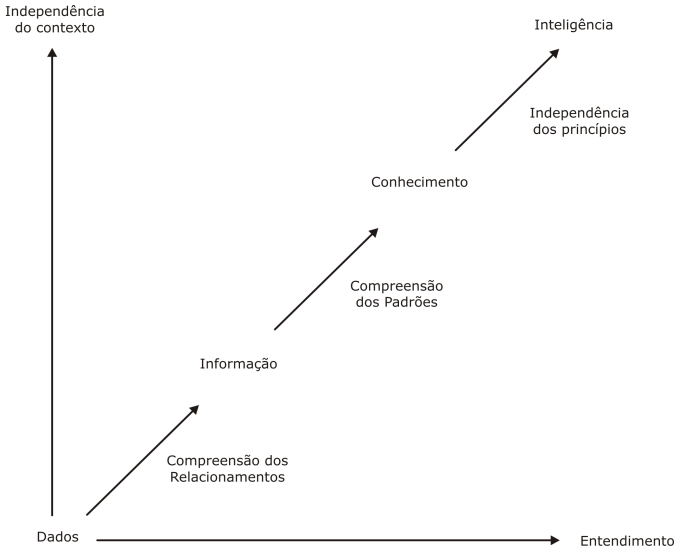
\includegraphics[width=0.65\textwidth]{Figuras/figura1.png}}
\caption{Relação entre dados, informação e conhecimento. Retirada de \cite{Rezende2003}.\label{fig:relação}}
\end{figure}

\section{Trajetória}
Trajetórias podem ser geradas por qualquer objeto que carregue um dispositivo, seja um pedestre, um carro ou até um animal. Cada trajetória tem um conjunto de propriedades que descrevem o movimento de um objeto. Segundo \cite{Giannotti2008}, tais propriedades podem ser divididas em características momentâneas e gerais. As momentâneas são o objeto em um determinado tempo t ou determinado momento de um tempo t. As características gerais referem-se a trajetória como um todo, como a forma geométrica, o tamanho total da trajetória, a duração e velocidade média e etc. Podemos definir então trajetória como um segmento espaço-temporal do caminho percorrido por um objeto como definido por \cite{Spaccapietra2008}.\\
\indent Na figura 2 demonstra exemplos de trajetórias brutas, de apenas um objeto e de vários objetos gerados por um dispositivo móvel, já na tabela 1 mostra como é a forma destes dados gerados.
\begin{figure}[!ht]
\center{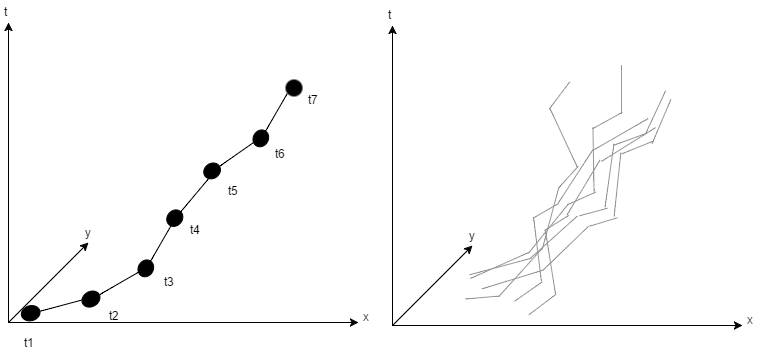
\includegraphics[width=0.65\textwidth]{Figuras/trajetorias.png}}
\caption{Uma trajetória e um conjunto de trajetórias. Adaptado de \cite{Giannotti2008}.\label{fig:trajetorias}}
\end{figure}

\begin{table}[!ht]
	\centering
		\caption{Tabela de trajetórias. Fonte:\cite{Bogorny2012}}	\label{tab:exemplo}
		\begin{tabular}{|c|c|c|}
			\hline  \textbf{Tid} &	\textbf{Posição(x,y)} &	\textbf{Tempo(t)} \\
			\hline 1 & 48.890018	2.246100	& 10:18	\\
			\hline 1 & 48.890020	2.246102	& 10:19	\\
			\hline 1 & 48.888880	2.248208	& 10:20	\\
			\hline 1 & 48.885732	2.255031	& 10:21	\\
			\hline 1 & 48.878433	2.283517	& 10:22	\\
            \hline 1 & 48.863214	2.279415	& 10:23	\\
			\hline 
		\end{tabular}
\end{table}

\subsection{Trajetória de objetos móveis}
Em \cite{Bogorny2012}, um aparelho de GPS pode ser configurado para gravar novos dados e consegue, por exemplo, gravar um ponto a cada segundo em que o objeto se move, um ponto a cada uma determinada distância em que o objeto se move ou ainda gravar pontos em determinado tempo \textit{t}, portanto a sequência dos pontos registrados para cada indivíduo é chamada de trajetória do objeto móvel.

\subsection{Ponto}
É um registro \textit{(x, y, t)}, no qual \textit{x} e \textit{y} são as coordenadas geográficas e \textit{t} é a identificação de tempo em que a coordenada foi coletada \cite{Bogorny2014}.

\subsection{Objeto}
É o objeto em movimento e que transporta um dispositivo móvel. Pode
ser uma pessoa, um carro, um animal, um robô etc \cite{Bogorny2014}.

\subsection{Dados semânticos}
São dados que buscam complementar as informações referentes às trajetórias, agregando valor, por exemplo, meio de transporte, velocidade, informações climáticas, entre outras \cite{Bogorny2014}.

\subsection{Enriquecimento semântico}
Em \cite{Furletti2013} é definido que o processo de agregar informações semânticas às trajetórias brutas é chamado enriquecimento semântico e, gera como saída uma trajetória semântica. Por exemplo, eventos, comportamento, objetivo, ambiente e atividade são formas de enriquecer uma trajetória bruta.

\subsection{Semântica em trajetórias}
Em trajetória bruta onde os dados são gerados por dispositivos móveis como GPS, é difícil extrair conhecimento interessante, entretanto se enriquecermos essas trajetórias com informações que agregam valor aos dados coletados pelos dispositivos de localização então a aplicação de extração de dados poderá ser mais eficiente em seus objetivos. Os benefícios de dados semanticamente enriquecidos podem alcançar resultados onde trajetórias brutas não permitiriam ter essa potencial visibilidade de prever ou tomar alguma decisão, por exemplo, se uma pessoa parou em um local por um determinado período de tempo (e.g. shopping, hotel, supermercado), permite observar qual o deslocamento de certas trajetórias como pessoas que estão hospedadas em um hotel e percorrem a cidade buscando por pontos turísticos e então a partir destes pontos quais restaurantes são mais visitados por essas pessoas.\\
\indent A idéia de agregar semântica às trajetórias de objetos móveis para facilitar a análise deste tipo de dado foi introduzida pela professora Vânia Bogorny e professor Luís Otávio Alvares ambos da UFSC em conjunto com o grupo da universidade de Hasselt, um pesquisador da Universidade de Buenos Aires e pesquisadores da EPFL. Foi criado um modelo para adicionar semântica às trajetórias, a fim de facilitar e otimizar consultas espaço-temporais \cite{alvares2007}, com o algoritmo SMoT. Os autores teve como base de seu trabalho o modelo conceitual para trajetórias elaborado pelo grupo de pesquisas do professor Spaccapietra, \cite{Spaccapietra2008}, chamado \textit{stop and moves} como \cite{Bogorny2012} diz em seu livro, uma trajetória bruta pode ser enriquecida com diferentes informações semânticas, de acordo com o contexto da aplicação e o problema que o usuário pretende resolver, ao tentarmos analisar uma trajetória bruta, será muito difícil encontrar algum padrão novo e interessante. Os padrões semânticos podem ser independentes de localização geográfica (se tiverem em lugares esparsos ou com poucos pontos ou trajetórias, em vez de locais densos, com muitos pontos ou trajetórias) e não apresentar nenhuma similaridade. Então padrões semânticos dificilmente serão extraídos de trajetórias brutas, depois de uma análise dos dados não se pode enriquecer semanticamente as trajetórias.\\
\indent	A área de pesquisa que considera contexto ou semântica em trajetórias ainda está na sua infância \cite{Bogorny2012}. 

\subsubsection{O modelo \textit{stops and moves}}
Até 2006 os estudos de trajetórias consideravam basicamente a geometria das trajetórias. No fim de 2006, publicado oficialmente em 2008, o trabalho de \cite{Spaccapietra2008}, criou um modelo conceitual para trajetórias chamado \textit{stops and moves}.\\
\indent Este modelo proposto define os \textit{stops} como as partes importantes da trajetória do ponto de vista da aplicação, ou seja, nas paradas de uma trajetória onde a mesma permaneceu por um determinado intervalo de tempo em lugar específico é onde o \textit{stop} tem mais importância, já que certas informações de semânticas podem dizer a qual lugar esta parada indica. Um \textit{move} é definido como a parte da trajetória (ou a subtrajetória) onde liga um \textit{stop} qualquer ate o seu próximo \textit{stop} consecutivo, e ainda a parte da trajetória até encontrar um \textit{stop} e a outra parte quando após o último \textit{stop} da trajetória, ou seja, entre o instante inicial e final da trajetória caso não exista nenhum \textit{stop}. Nesse modelo, todas as partes da trajetória que não são \textit{stops} representam \textit{moves}.\\
\indent Ao considerarmos, por exemplo, um hotel como um \textit{stop}, onde o objeto móvel é uma pessoa que ficou um determinado tempo \textit{t} neste hotel, no ponto de vista da aplicação o objeto ficou parado no \textit{stop}, pois se mostra relevante a permanência da pessoa no hotel por um determinado tempo.\\
\indent O processo de \textit{stops and moves} é muito similar à engenharia reversa de banco de dados, neste processo precisamos dos dados para que o modelo \textit{stops and moves} seja gerado a partir desses dados.\\
\indent \cite{Spaccapietra2008} define \textit{stops and moves} como a seguir: 

\begin{itemize}
\item \textit{Stop}:
	\begin{itemize}
    \item O usuário explicitamente define parte do percurso em início e término para representar um \textit{stop}.
    \item O tempo de um percurso de início e término é um intervalo de tempo não nulo.
    \item O tempo de todas as paradas são separados, ou seja, o tempo de duas paradas são sempre disjuntas.
    \end{itemize}
\item \textit{Move:}
	\begin{itemize}
    \item Uma parte é delimitada por duas extremidades que representam dois \textit{stops} consecutivos, ou o início e o primeiro \textit{stop}, ou o último \textit{stop} e término, ou [início, término] (sem \textit{stops}).
    \item O tempo de um percurso de início e término é um intervalo de tempo não nulo.
    \item O alcance espacial da trajetória de início e término de um intervalo é o espaço-temporal de uma linha (não um ponto) definido pela função da trajetória.
    \end{itemize}
\end{itemize}

\subsubsection{Trajetória semântica}
Trajetória bruta tem suas limitações citadas ao longo de deste trabalho, trabalhar com trajetória semântica tem vantagem por ser mais receptivas e compreendidas, onde são fáceis de perceber a diferença entre essas trajetórias, pois semânticas são carregadas com informações ao longo da trajetória, abaixo na figura 3 existem 3 trajetórias (1) Bruta e (2) e (3) semânticas, é fácil diferenciá-las, porém na trajetória 2 se trata de uma aplicação de turismo, pois os pontos de interesse são lugares onde faz parte do contexto da aplicação. Já na trajetória 3 a semântica faz parte de uma aplicação de trânsito e as partes mais interessantes são partes onde se tem o maior movimento de veículos parados. Pontos importantes da trajetória que identificamos na figura 3 onde nas trajetórias (2) e (3) são lugares marcados com cores, significa pontos de \textit{stops}, e o restante dessas trajetórias são \textit{moves}.  

\begin{figure}[!ht]
\center{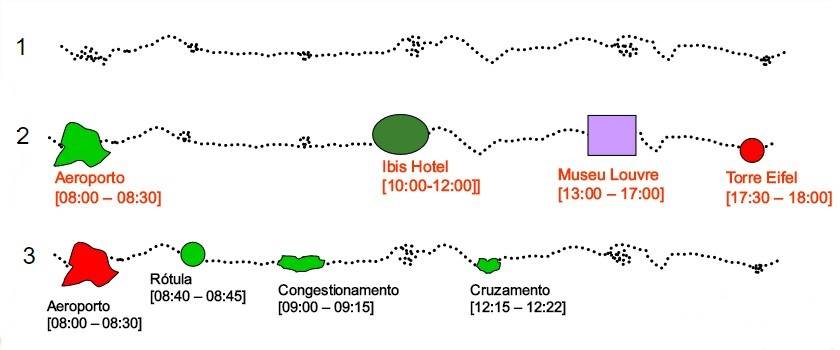
\includegraphics[width=0.65\textwidth]{Figuras/trajetorias2.jpg}}
\caption{Exemplos de trajetórias:(1) bruta, (2) e (3) semânticas. Retirada de \cite{Bogorny2012}.\label{fig:figura}}
\end{figure}

\section{O algoritmo SMoT}
A tarefa desempenhada por este algoritmo é verificar se cada ponto de uma trajetória bruta \textit{T} tem uma intersecção com a área geométrica de um candidato a \textit{stop}, ou seja, essa área geométrica são objetos geográficos relevantes para a aplicação. Se existe a validação de intersecção em algum ponto da trajetória, então o algoritmo verifica a duração da intersecção, que deve ser igual ou superior que o tempo mínimo estabelecido para aquele tipo de objeto geográfico, então o objeto será considerado um \textit{stop}, em caso de o tempo não ter o seu mínimo atingido aquele objeto geográfico não pode ser considerado um \textit{stop} então não é adicionado aos \textit{stops} encontrados. Este algoritmo possui como entrada um conjunto de trajetórias e um conjunto de candidatos à \textit{stop}, tendo como saída uma tabela de \textit{stops} e uma tabela de \textit{moves}.
No Algoritmo 1 é apresentado um pseudocódigo de extração de \textit{stops and moves}, proposto por \cite{alvares2007}. \\

\begin{algorithm}[H]
   \SetAlgoLined
   \Entrada{$T, A$} 
%  \Saida{Número esperado de nodos atingidos}
   \Inicio{
    $S \leftarrow new  Stops()$\ \\
    $M \leftarrow new  Moves()$\ \\
    \Para{$cada \,\, trajetória \,\, t \in T$}{
   	 $i \leftarrow 0$\ \\
     $previousStop \leftarrow null$\ \\
      \Enqto{$i \le size(t)$}{
      	\Se{$\exists\,\,(Rc,\Delta c) \in A \mid geometria(t[i]) \cap Rc$}{
        	$enterTime \leftarrow time(t[i])$\ \\
            $i++$\ \\
        \Enqto{$geometria(t[i]) \cap Rc)$}{
        	$i++$\
        }
        $i--$\ \,\, , \,\,
        $leaveTime \leftarrow time(t[i])$\ \\
        \Se{$leaveTime - enterTime \ge \Delta c$}{
        	$stop \leftarrow (t,Rc,enterTime,leaveTime)$\ \\
            $S.add(stop)$\ \\
            $move \leftarrow (t,previousStop,stop,previousStop.leaveTime,enterTime)$\ \\
            $M.add(move)$\ \\
            $previousStop \leftarrow stop$\
         }
        }
        $i++$\ \,\, ,\,\,
        $j \leftarrow 1$\ \\
        \Enqto{$(i+j \le size(t))\,\, and\,\, (t[i+j]-t[i] < min\,\, \Delta c\, (A))$}{
        	$j++$\
        }
        \Se{$\not\exists \,\,(Rc,\Delta c) \in A \mid geometria(t[i+j-1]) \,\, \cap Rc$}{
        $i \leftarrow i+j$\
        }
   	  }
      \Se{$ t[i-1]\,\, not \in previousStop$}{
      $move \leftarrow (t,previousStop,null,previousStop.leaveTime,time(t[i-1]))$\ \\
      $M.add(move)$\
      }
    }
   }
   \label{algoritmo1}
   \caption{\textsc{Pseudocódigo SMoT}}
\end{algorithm}

O algoritmo verifica para cada ponto de uma trajetória t se cruza com a geometria de um candidato a\textit{ stop Rc} (linha 8). Em caso afirmativo, o algoritmo avalia a duração da intersecção tem, pelo menos, um limite igual a \textit{$\Delta$c} (linha 15). Se esse é o caso esse \textit{stop} é gravado. Note que quando usamos \textit{t} e \textit{Rc} como parâmetros (por exemplo, linha 16), usamos e atribuímos na realidade um identificador de chave estrangeira e não toda uma estrutura de dados. \\
\indent Esse método de \textit{stops and moves} tem um nome mais específico chamado IB-SMoT \textit{(Intersection-Based Stops and Moves of Trajectories)} que por meio de sobreposição dos principais pontos de uma trajetória bruta, respeitando o tempo limite mínimo de intersecção do ponto, se obtêm a partir de locais preestabelecidos pelo usuário candidatos de \textit{stops} na trajetória. Na figura 4 o algoritmo IB-SMoT encontrou três candidatos a \textit{stop} na trajetória.

\begin{figure}[!ht]
\center{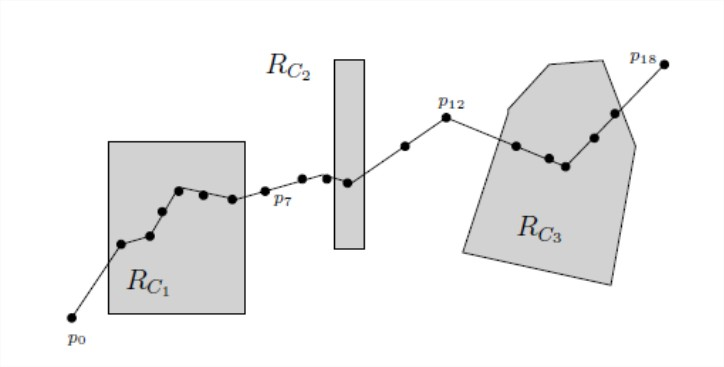
\includegraphics[width=0.65\textwidth]{Figuras/IB-SMOT.jpg}}
\caption{Exemplo de IB-SMOT com \textit{stops} encontrados.\cite{alvares2007}\label{fig:IB-SMOT}}
\end{figure}

\subsection{Padrões de movimentos em trajetórias}
Um movimento relativo de várias trajetórias de objetos móveis pode auxiliar a encontrar certos padrões em trajetórias como recorrências e encontros que é o principal foco deste trabalho, em \cite{laube2005finding} descreve esses padrões de movimentos como a seguir:
\begin{itemize}
\item Encontro é um determinado número de trajetórias dentro de um raio \textit{R}, onde um conjunto \textit{m} de trajetórias em um determinado intervalo \textit{i} se move em uma mesma direção, passando por uma determinada área fazendo intersecção com o intervalo de raio \textit{R} tendo uma mesma velocidade.
\item Convergência é um conjunto \textit{m} de trajetórias que interceptam uma mesma região de raio \textit{R}, não necessariamente no mesmo momento.
\end{itemize}

Observe a diferença entre estes dois padrões de movimento, na figura 5 o padrão é de encontro, onde as trajetórias têm a mesma direção e velocidade e ficam dentro do raio um certo tempo. Já na figura 6 o padrão é de convergência, onde as trajetórias vêm de todos os sentidos na mesma direção, porém não ao mesmo tempo.

\begin{figure}[ht]
\center{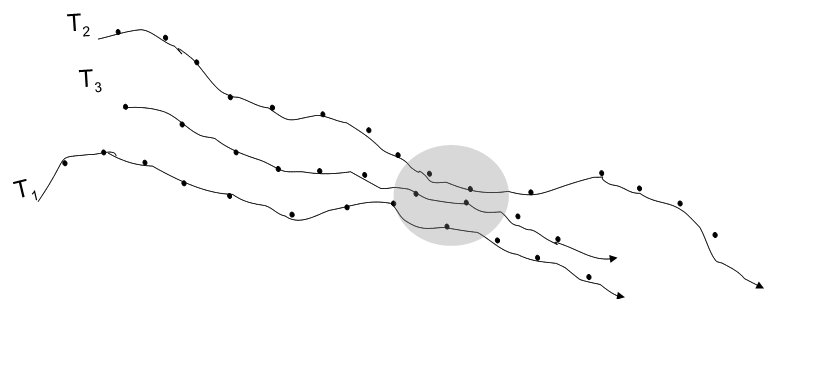
\includegraphics[width=0.65\textwidth]{Figuras/encontro.png}}
\caption{Exemplo de encontro.\cite{Bogorny2012}\label{fig:encontro}}
\end{figure}

\begin{figure}[ht]
\centering{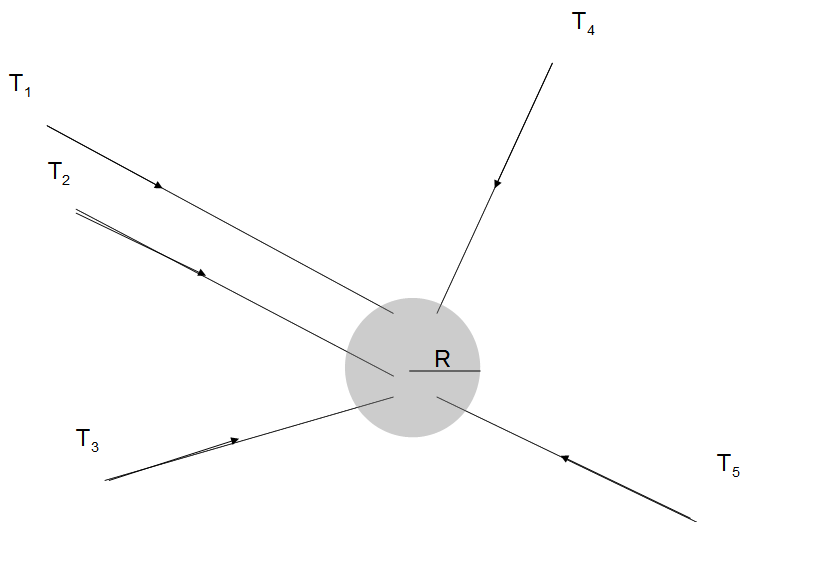
\includegraphics[width=0.65\textwidth]{Figuras/convergencia.png}}
\caption{Exemplo de convergência.\cite{Bogorny2012}\label{fig:convergencia}}
\end{figure}

\chapter{Trabalhos relacionados}
Entre os últimos artigos publicados em 2015 sobre enriquecimento de trajetórias está o trabalho de \cite{sublime2015}, que tem características específicas que permitem a extração de informações semântica sobre dados geográficos de imagens de alta resolução, esse tipo de extração de semântica é muito usado quando os dados não são obtidos via objetos móveis, já que se obtêm a semântica a partir de dados. Porém com estes dados, são gerados mapas atualizados que são proveitosos para aplicar semântica em trajetórias brutas de objetos móveis. Os estudos em torno de trajetórias semânticas e enriquecimento semântico têm tido um grande avanço nos últimos anos.\\
\indent No trabalho de \cite{alvares2007}, o enriquecimento de trajetórias é feito com informações geográficas para simplificar consultas que são complexas, então é proposto um pré-processamento de modelo de dados para adicionar informações semânticas as trajetórias.\\
\indent Em \cite{laube2005finding}, é introduzido o estudo de comportamento de movimentos de trajetórias, onde o autor explica como se obtêm cada tipo de movimento o que vem a ser proveitoso para este trabalho, o padrão de encontro que é exemplificado no livro é o mais complexo de se calcular, por que temos que medir o intervalo de tempo de todas as trajetórias que passam em um determinado raio \textit{R}.\\
\indent Em \cite{Bogorny2012} uma trajetória bruta pode ser enriquecida com diferentes informações semânticas de acordo com o contexto da aplicação e o problema que o usuário pretende resolver.\\
\indent Neste trabalho é utilizado o método de enriquecimento de trajetórias onde usaremos informações geográficas para conflitar com as trajetórias e dizer se são pontos de \textit{stops} através do algoritmo de \textit{stops and moves}, tendo esses dados enriquecidos semanticamente vai ser implementado um algoritmo que detecta encontros em trajetórias a partir de um raio dado e um tempo de permanência mínimo em cada \textit{stop}.

\chapter{Plano de atividades para o TCC II}
Para a continuação deste trabalho o cronograma abaixo deve ser seguido.

\begin{table}[!ht]
	\centering
		\caption{Plano de atividades para o TCC II}	\label{tab:plano}
		\begin{tabular}{|c|c|c|c|c|c|c|}
			\hline  \textbf{Atividades} &	\textbf{Março} &	\textbf{Abril} & \textbf{Maio} & \textbf{Junho} & \textbf{Julho} \\
			\hline 1 & $\checkmark$ 	& & & & 	\\
			\hline 2 & $\checkmark$	& & & & 	\\
			\hline 3 & 	&$\checkmark$ &$\checkmark$ & & 	\\
			\hline 4 & 	&$\checkmark$ &$\checkmark$ &$\checkmark$ & 	\\
			\hline 5 & 	&$\checkmark$ &$\checkmark$ &$\checkmark$ & 	\\
            \hline 6 &  & & & &$\checkmark$ 	\\
			\hline 
		\end{tabular}
\end{table}
\begin{enumerate}
\item Busca de uma base de dados correta para a aplicação.
\item Evidenciar o contexto semântico a ser aplicado.
\item Implementar o algoritmo SMoT.
\item Implementar o algoritmo que detecta encontros.
\item Análise e comparação dos resultados.
\item Documentação total do trabalho.
\item Apresentação do trabalho.
\end{enumerate}

\chapter{Conclusão}
A forma de enriquecer semânticas de objetos móveis, é uma área de pesquisa que cresce cada vez mais, e a produção de dispositivos móveis cresce de uma forma muito agressiva no mercado resultando em grandes volumes de dados geográficos, porém aonde aplicar todos os métodos que vimos neste trabalho e obter resultados significativos, isso ainda está em sua infância. \\
\indent	Em aplicações onde se usam dados gerados por dispositivos móveis, deve ser feito um estudo muito bem-feito para enriquecer suas trajetórias, onde o contexto da aplicação depende muito na execução do algoritmo para obter excelentes resultados.\\
\indent	A proposta deste trabalho é trabalhar com dados fornecidos de trajetórias brutas e aplicar o método SMoT para enriquecê-las semanticamente e posteriormente analisar essas rotas e indicar em quais pontos houve encontros, independente de qual objeto gerou tais rotas.

%\begin{itemize}
%\item Contextualização e Motivação; 
%\item Definição do problema; 
%\item Justificativas;
%\item Objetivos:  Geral e específicos;
%\item Metodologia e
%\item Organização do documento.
%\end{itemize}

%\subsection{Sobre os Títulos e Capítulos}

%As demais subdivisões do texto (seções, subseções, etc) ... 

%\subsubsection{Título de Subseção}
%Veja aqui um exemplo de citaçao direta \cite{memoir}.


% ----------------------------------------------------------
% Capitulo com exemplos de comandos inseridos de arquivo externo 
% ----------------------------------------------------------

% ---
% Capitulo de revisão de literatura
% ---
%\chapter{Revisão Bibliográfica}

% ---
%\section{Introdução}
% ---

% ---
% primeiro capitulo de Resultados
% ---
%\chapter{Resultados}

% ---
% Finaliza a parte no bookmark do PDF, para que se inicie o bookmark na raiz
% ---
\bookmarksetup{startatroot}% 
% ---

% ---
% Conclusão
% ---

% ----------------------------------------------------------
% ELEMENTOS PÓS-TEXTUAIS
% ----------------------------------------------------------
%\postextual


% ----------------------------------------------------------
% Referências bibliográficas
% ----------------------------------------------------------
%\bibliographystyle{plain}
\bibliography{references}

% ----------------------------------------------------------
% Glossário
% ----------------------------------------------------------
%
% Consulte o manual da classe abntex2 para orientações sobre o glossário.
%
%\glossary

% ----------------------------------------------------------
% Apêndices
% ----------------------------------------------------------

% ---
% Inicia os apêndices
% ---
%\begin{apendicesenv}

% Imprime uma página indicando o início dos apêndices
%\partapendices

% ----------------------------------------------------------
%\chapter{Título de Apêndice}
% ----------------------------------------------------------


% ----------------------------------------------------------
%\chapter{Título do Apêndice}
% ----------------------------------------------------------


%\end{apendicesenv}
% ---


% ----------------------------------------------------------
% Anexos
% ----------------------------------------------------------

% ---
% Inicia os anexos
% ---
%\begin{anexosenv}

% Imprime uma página indicando o início dos anexos
%\partanexos

% ---
%\chapter{Título do Anexo}
% ---

%\end{anexosenv}

\end{document}